\documentclass[11pt]{article}

\usepackage{report}
\usepackage{algpseudocode}
\usepackage{algorithm}
\usepackage[utf8]{inputenc} % allow utf-8 input
\usepackage[T1]{fontenc}    % use 8-bit T1 fonts
\usepackage[colorlinks=true, linkcolor=black, citecolor=blue, urlcolor=blue]{hyperref}       % hyperlinks
\usepackage{url}            % simple URL typesetting
\usepackage{booktabs}       % professional-quality tables
\usepackage{amsfonts}       % blackboard math symbols
\usepackage{nicefrac}       % compact symbols for 1/2, etc.
\usepackage{microtype}      % microtypography
\usepackage{lipsum}		% Can be removed after putting your text content
\usepackage{graphicx}
\graphicspath{ {./images/} }
\usepackage{natbib}
\usepackage{doi}
\setcitestyle{aysep={,}}
\usepackage{array}

\usepackage{listings}

\usepackage{xcolor}
\definecolor{codegreen}{rgb}{0,0.6,0}
\definecolor{codegray}{rgb}{0.5,0.5,0.5}
\definecolor{codeorange}{rgb}{1,0.49,0}
\definecolor{backcolour}{rgb}{0.95,0.95,0.96}

\lstdefinestyle{mystyle}{
    backgroundcolor=\color{backcolour},   
    commentstyle=\color{codegray},
    keywordstyle=\color{codeorange},
    numberstyle=\tiny\color{codegray},
    stringstyle=\color{codegreen},
    basicstyle=\ttfamily\footnotesize,
    breakatwhitespace=false,         
    breaklines=true,                 
    captionpos=b,                    
    keepspaces=true,                 
    numbers=left,                    
    numbersep=5pt,                  
    showspaces=false,                
    showstringspaces=false,
    showtabs=false,                  
    tabsize=2,
    xleftmargin=10pt,
}

\lstset{style=mystyle}


\title{CT2109 - Object Oriented Programming: Data Structures \& Algorithms}

\author{Andrew Hayes\\
\AND
\AND
\AND
\AND
\AND
	2BCT\\
\AND
    University of Galway\\
}

% Uncomment to remove the date
% \date{February 2022}

% Uncomment to override  the `A preprint' in the header
\renewcommand{\headeright}{Object Oriented Programming: Data Structures \& Algorithms}
\renewcommand{\undertitle}{Object Oriented Programming: Data Structures \& Algorithms}
\renewcommand{\shorttitle}{}

%%% Add PDF metadata to help others organize their library
%%% Once the PDF is generated, you can check the metadata with
%%% $ pdfinfo template.pdf
% \hypersetup{
% pdftitle={A template for the arxiv style},
% pdfsubject={q-bio.NC, q-bio.QM},
% pdfauthor={David S.~Hippocampus, Elias D.~Striatum},
% pdfkeywords={First keyword, Second keyword, More},
% }

\begin{document}
\maketitle

\newpage
\tableofcontents
\thispagestyle{empty}
\setcounter{page}{1}

\newpage
\section{Abstract Data Types}  
An \textbf{Abstract Data Type (ADT)} is an abstract model of a data structure that specifies the data stored \& oeprations that may be performed on the data. 
An ADT specifies \textit{what} each operation does, but not \textit{how}. 
In object-oriented languages such as Java, this naturally corresponds to an \textbf{interface definition}. 
An ADT is \textit{realised} as a concrete data structure. 
In Java, this is a class that \textbf{implements} the interface. 

\begin{center}
    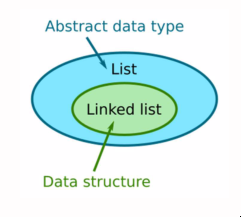
\includegraphics[width=0.3\textwidth]{adt.png}
\end{center}

\textbf{Composite ADTs} are used manage \textit{collections} of data, e.g., Arrays, Lists, Stacks, Queues, Hash Tables, etc. 

\subsection{Stacks \& Queues}
\textbf{Stacks} \& \textbf{Queues} are linearly ordered ADTs for list-structured data. 

\subsubsection{Stacks}
A \textbf{Stack} is a last in, first out (LIFO) data structure. 
No sort order is assumed.
Items can only enter or leave via the \textit{top} of the stack. 
Items can be \textbf{pushed} \& \textbf{popped} to add \& remove. 
Example applications of a stack include processing nested structures or the ``undo'' operation in an editor.
Objects stored in a stack are a \textit{finite sequence} of elements of the \textbf{same type}. 

Stacks have few operations. 
For a stack \verb|s|, node \verb|n|, \& boolean value \verb|b|:
\begin{itemize}
    \item \verb|s.push(n)| - Place item \verb|n| on top of the stack. 
    \item \verb|s.pop()| $\rightarrow$ \verb|n| - Remove top item from the stack \& return it. 
    \item \verb|s.top| $\rightarrow$ \verb|n| - Examine the top item on the stack without removing it. 
    \item \verb|s.isEmpty()| $\rightarrow$ \verb|b| - Returns \verb|b = true| if the stack is empty. 
    \item \verb|s.isFull()| $\rightarrow$ \verb|b = true| if the stack is full (relevant if storage is limited). 
\end{itemize}

Java has a built-in stack interface from \verb|java.util.Stack|. 
However, we will look at making our own for the sake of learning. 
Our stack implementation may look something like this:
\begin{lstlisting}[language=java]
public interface Stack {
    public void push(Object n);
    public Oject pop();
    public Object top();
    public boolean isEmpty();
    public boolean isFull();
\end{lstlisting}

Other stack operations include \verb|size()| \& \verb|makeEmpty()|. 
We could implement this stack using an array, linked list, or other storage type. 

\subsubsection{Queues}
A \textbf{Queue} is a first in, first out (FIFO) data structure. 
No sort order is assumed.
Items enter at the rear of the queue, and leave at the front of the queue. 
Items can be \textbf{enqueued} \& \textbf{dequeued} to add \& remove them from the queue. 
Example applications of a queue include ensuring ``fair treatment'' to each of a list of pending tasks (first come, first served) 
or simulation: modelling \& analysis of real-world problems.
Objects stored in a queue are a finite sequence of elements of the same type. 
The item at the front of the queue has been in the queue the longest, while the item at the rear has entered the queue most recently. 

Queues have few operations. 
For a queue \verb|q|, element \verb|e|, \& boolean value \verb|b|: 
\begin{itemize}
    \item \verb|q.enqueue(e)| - Place \verb|e| at the rear of \verb|q|, assuming there is space. 
    \item \verb|q.dequeue()| $\rightarrow$ \verb|e| - Remove fron item \verb|e| from \verb|q| and return it. 
    \item \verb|q.front()| $\rightarrow$ \verb|e| - Returns front element \verb|e| without removing it. 
    \item \verb|q.isEmpty()| $\rightarrow$ \verb|b| - Returns \verb|b = true| if the queue is empty. 
    \item \verb|q.isFull()| $\rightarrow$ \verb|b| - Returns \verb|b = true| if the queue is full. 
\end{itemize}

With an array implementation of a queue, items must be ``shuffled'' towards the front after a \textit{dequeue}. 
Note that with an array implementation, once \verb|rear| becomes equal to $N-1$, no further items can be enqueued (array space limitation). 

\subsection{Linked Lists}
A \textbf{Linked List} is an abstract data type which stores an arbitrary-length list of data objects as a sequence of \textit{nodes}. 
Each node consists of data and has a \textbf{link} to the next node. 
Each node, excepting the last, is links to a \textbf{successor node}. 

\begin{center}
    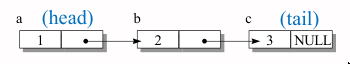
\includegraphics[width=0.6\textwidth]{ll.png}
\end{center}

Characteristics of Linked Lists:
\begin{itemize} 
    \item   \textbf{Self-referential} structure type - Every node has a pointer to a node of the same type. 
    \item   Very useful for \textbf{dynamically} growing/shrinking lists of data. 
    \item   Compared to arryas, drastically reduces the effort required to add/remove items from the middle of the list.
    \item   Solves the potential problem of \textbf{overflow} that arrays have. 
    \item   \textbf{Sequential access} - It is \textbf{inefficient} to retrieve an element at an arbitrary position, relative to an array. 
\end{itemize}

\subsubsection{Implementation of Linked Lists}
We define a \textbf{Node} class, with members \textbf{data} (whichever variables are required) \& \textbf{next} (reference to another Node object). 

Each node occcurrence is linked to a succeeding occurence by way of the member \textbf{next}. 
If \verb|next| is \verb|null|, then there is no item after this node in the list (termed the \textbf{tail} node). 
The starting point for the list is the \textbf{head} node. 
We can trace from the head node to any other node. 

\begin{center}
    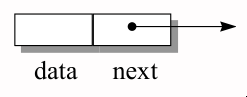
\includegraphics[width=0.3\textwidth]{node.png}
\end{center}

\begin{lstlisting}[language=Java] 
public class Node {
    // instance variables 
    private Object element; 
    private Node next; 

    // creates node with null refs to its element \& next node 
    public Node() {
        this(null, null);
    } 

    // creates node with the given element & next node 
    public Node(Object e, Node n) {
        element = e; 
        next = n; 
    } 

    // accessor methods 
    public Object getElement() {
        return element;
    } 
    public Node getNext() {
        return next; 
    }

    // mutator methods 
    public void setElement(Object newElem) {
        element = newElem; 
    } 
    public void setNext(Node newNext) {
        next = newNext;
    }
}
\end{lstlisting}

Generally, we don't create nodes manually, rather we just supply element data to a method which keeps track of the current position in the list.

Typical methods in a Linked List ADT include:
\begin{itemize}
    \item   \verb|long size()| - Returns the size of the list. 
    \item   \verb|boolean isEmpty()| - Returns \verb|true| if the list is empty, \verb|false| otherwise. 
    \item   \verb|Object getCurr()| - Returns the element at the current position. 
    \item   \verb|boolean gotoHead()| - Sets the current position to \verb|head|, returning \verb|true| if successful. 
    \item   \verb|boolean gotoNext()| - Moves to the next position, returning \verb|true| if successful.
    \item   \verb|void insertNext(Object el| - Creates a new node after the current node. 
    \item   \verb|void deleteNext()| - Removes the node after the current node. 
    \item   \verb|void insertHead(Object el)| - Creates a new node at the head. 
    \item   \verb|void deleteHead()| - Removes the head node. 
\end{itemize}

\subsubsection{Singly Linked List Class}
A \textbf{singly linked list} is one in which each node links to a \textit{single} other node. 

The Singly Linked List Class should store the head of the list \& the current position. 
For efficiency, it also keeps track of the current size of the list (alternatively, we could just count its nodes when needed). 

\begin{lstlisting}[language=Java]
public class SLinkedList {
    protected Node head;    // head node of the list
    protected Node curr;    // current position in list 
    protected long size;    // number of nodes in the list 

    // default constructor which creates an empty list
    public SLinkedList() {
        curr = head = null; 
        size = 0; 
    } 

    // insert, remove, & search methods go here 
}
\end{lstlisting}

\section{Algorithm Analysis}
All algorithms take CPU \textbf{time} \& \textbf{memory} space. 
Often, we can make tradeoffs, choosing algorithm variants that either user more memory, or more CPU. 
If the memory space requirements of an algorithm are large, the program may use disk sawp space rather than RAM, which is much slower. 
If the memory requirements are too large, then the program cannot run. 
Often, we identify the algorithms that don't require ``too much'' spaace, and then choose the one with the lowest 
CPU requirements. 
The purpose of algorithm analysis is comparing the time \& space requirements of various algorithms. 

``Why not just run the algorithm and measure the time \& space used?'' - 
While this is sometimes done when theoretical analysis is difficult, it is better to be able to evaluate 
algorithms ``on paper'' without first having to implement, debug, and test them all.
It's important to have a measure that's \textit{independent} of particular computer configurations and to be able to  
compare algorithms reliably, without being influenced by variations in implementation. 
We want to understand how an algorithm will perform on large problems and identify ``hot spots'' to give our attention 
to when developing \& optimising programs. 

\subsection{Algorithm Analysis Basics}
\textbf{Theoretical Analysis} uses a high-level \textit{pseudocode} description of the algorithm instead of a real 
implementation, and characterises run-time as a function of input size $n$. 
This function specifies the \textbf{order of growth} of rate of runtime as $n$ increases. 
Theoretical analysis takes into account all possible inputs and evaluates speed independent of hardware or software. 

\subsubsection{Counting Primitive Operations}
The basic approach is deriving the function for the \textbf{count of the primitive operations}. 
The primitive operations are the individual steps performed by a program. 
We assume that each step takes the same amount of time and examine any terms that control repetition. 

Example: Algorithm to find the largest element of an array. 
We count the maximum number of operations as function of array size $n$.
\begin{lstlisting}
Algorithm arrayMax(A, n)            // Number of Operations
    currentMax = A[0]               // 2  
    for i = 1 to n -1 do            // 2n 
        if A[i] > currentMax then   // 2(n-1)
            currentMax = A[i]       // 2(n-1)
            {increment coutner i}   // 2(n-1)
    return currentMax               // 1
                                    // Total: 8n-3
\end{lstlisting}

We could consider the \textbf{average}, \textbf{best}, or \textbf{worst} case. 
Usually, we analyse the worst case, as we want our algorithms to work well even in bad cases. 
The average case is quite important too, if different from the worst case.
These counts are the basis of (big) O notation.

\subsection{O Notation} 
The basic approach to \textbf{O Notation} involves deriving an expression for the count of basic operations (as 
discussed). 
We focus on the \textit{dominant term}, and ignore constants. 
E.g., $O(5n^2 + 1000n -3) \rightarrow O(n^2)$.
Since contants \& low-order terms are eventually dropped, we can disregard them when counting primitive operations. 

O Notation is used for \textbf{asymptotic analysis of complexity} - the trend in the algorithms runtime as $n$ 
gets large. 
We look at the \textbf{order of magnitude} of the number of actions, independent of computer/compiler/etc. 

Note: We specifically care about the \textbf{tightest} upper bound. 
Technically speaking, an algorithm that is $O(n^2)$ is also $O(n^3)$, but the former is more informative.
The function specified in O notation is the \textbf{upper bound} on the behaviour of the algorithm being analysed. 
This can be the best/average/worst case behaviour.

Example: Let $f(n) = 6n^4 -2n^3 + 5$. 
Apply the following rules:
\begin{itemize}
    \item   If $f(n)$ is a sum of several terms, then only the one with largest rate of growth is kept. 
    \item   If $f(n)$ is a product of several factors, any constants that do not depend on $n$ are ommitted. 
\end{itemize}
Thus, we say that $f(n)$ has a ``big-oh'' of $(n^4)$. 
We can write $f(n)$ is $O(n^4)$. 

\subsubsection{Important Functions Used in O Notation} 
Functions commonly used include:
\begin{itemize}
    \item   \textbf{Constant:} $O(1)$. 
    \item   \textbf{Logarithmic:} $O($log$n)$.
    \item   \textbf{Linear:} $O(n)$. 
    \item   \textbf{n-Log-n:} $O(n$log$n)$. 
    \item   \textbf{Quadratic:} $O(n^2)$. 
    \item   \textbf{Cubic:} $O(n^3)$. 
    \item   \textbf{Exponential:} $(1^n)$. 
\end{itemize}

Notes:
\begin{itemize}
    \item   By convention, all logs are base 2 unless otherwise stated. 
    \item   Two algorithms having the same complexity doesn't been that they are exactly the same, it means that their 
            running times will be \textit{proportional}.
\end{itemize}


\begin{center}
    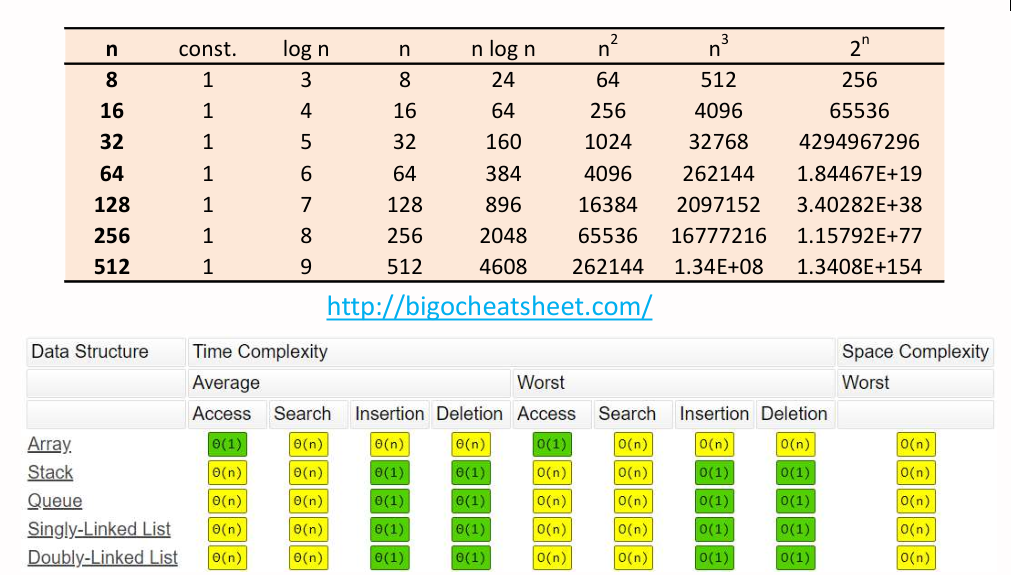
\includegraphics[width=0.8\textwidth]{comparisonoffunctions1.png}
\end{center}

\begin{center}
    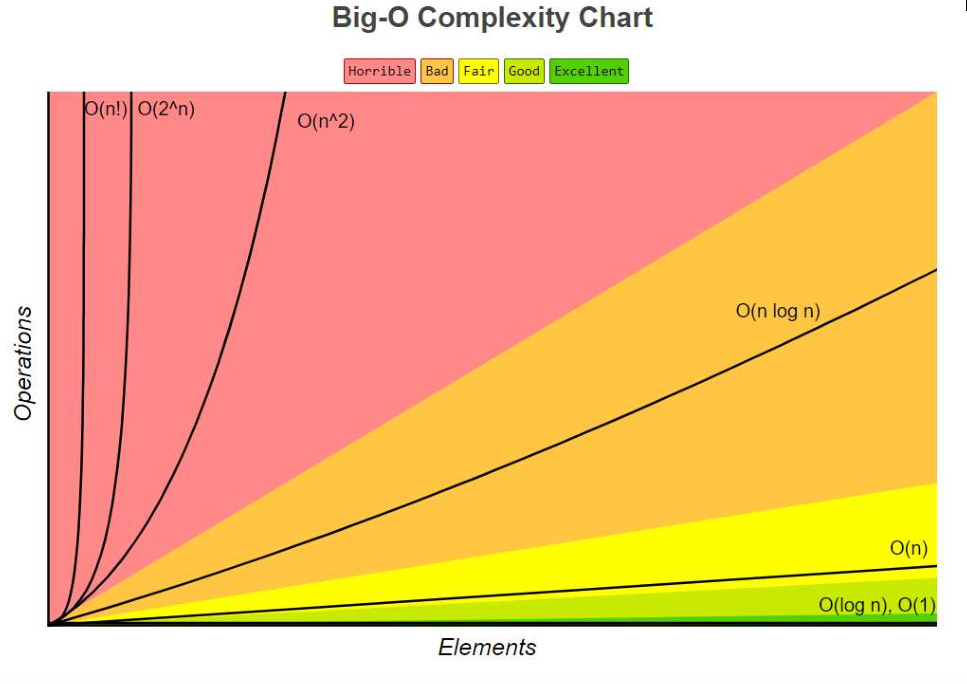
\includegraphics[width=0.8\textwidth]{comparisonoffunctions2.png}
\end{center}

\subsubsection{Efficiency \& O Notation}
\begin{itemize}
    \item   \textbf{Constant:} Most efficient possible, but only applicable to simple jobs. 
    \item   \textbf{Logarithmic, Linear, \& n-Log-n:} If an algorithm is described as ``efficient'', this usually means 
            $O($log$n)$ or better.
    \item   \textbf{Quadratic \& Cubic:} Not very efficient, but polynomial algorithms are usually considered ``tractable'' 
            (acceptable for problems of reasonable size). 
    \item   \textbf{Exponential:} Very inefficient. Problems that (provably) require an algorithm of O greater than 
            polynomial complexity are called ``\textbf{hard}''.
\end{itemize}

\subsection{Recursion Review}
Methods can call other methods, but they can also call themselves, either directly, or indirectly, via 
another method.
This creates a type of loop called \textbf{recursion}. 

Iteration can be used anywhere that you can use recursion. 
Sometimes, recursion can be a more elegant solution, if it reflects the way that the problem is usually thought 
about, as we aim to use the most intuitive representation of the problem.
Recursion can make complexity analysis easier in some cases.

The drawbacks of recursion include:
\begin{itemize}
    \item   Inefficient use of the function: Large amount of concurrent, deeply nested method calls. 
    \item   If done naively, the number of calls can explode.
    \item   Depending on the algorithm, we need to take care not to recompute values unnecessarily. 
\end{itemize}

\section{Dynamic Programming}
The basic idea of \textbf{Dynamic Programming} is to solve complex problems by breaking them into simpler 
sub-problems. 
When a solution to a sub-problem is found, store it (``memo-ize'') so that it can be re-used without 
recomputing it. 
Combine the solutions to the sub-problems to get the overall solution. 

This is particularly useful when the number of repeating sub-problems grows exponentially with the problem 
size.

In general, dynamic programming takes problems that appear exponential and produces polynomial-time algorithms 
for them.
The trade-off in dynamic programming is between \textit{storage} \& \textit{speed}.
Dynamic programming is widely used in heuristic optimisation problems.

For Dynamic Programming, the problem structure requires three components:
\begin{enumerate}
    \item   \textbf{Simple sub-problems:} Must be able to break the overall problem into indexed sub-problems 
            \& sub-sub-problems. 
    \item   \textbf{Sub-problem decomposition:} Optimal/correct solution to the overall problem must be 
            composed from sub-problems.
    \item   \textbf{Sub-problem overlap:} So that elements can be re-used.
\end{enumerate}

The basic steps in the approach to DynProg: 
\begin{enumerate}
    \item   Set up the overall problem as one that is decomposable into overlapping sub-problems that can 
            be indexed. 
    \item   Solve the sub-problems as they arise and \textbf{store solutions} in a table.
    \item   Derive the overall solution from the solutions in the table.
\end{enumerate}

\subsection{More Big Greek Letters}
$O(n$log$n)$ (``Big Oh''): 
\begin{itemize}
    \item   Upper bound on asymptotic complexity. 
    \item   In this case, there is a constant $c_2$ such that $c_2 n$log$n$ is an upper bound on 
            asymptotic complexity. 
\end{itemize}

$\Omega(n$log$n)$ (``Big Omega''):
\begin{itemize}
    \item   Specifies a lower bound on asymptotic complexity. 
    \item   In this case, the algorithm has a lower bound of $c_1 n$log$n$. 
\end{itemize}

$\Theta(n$log$n)$ (``Big Theta''): 
\begin{itemize}
    \item   Specifies the upper \& lower bounds.
    \item   In this case, there exist two constants, $c_1$ \& $c_2$, such that $c_1n$log$n < f(n) < c_2n$log$n$.
\end{itemize}

Of these, $\Theta()$ makes the strongest claims: It specifies that the rate of growth is no better and no 
worse than some level. 
Requires additional analysis relative to $O$. 

There are also some others that are common in Mathematics but not in Computer Science: 
\begin{itemize}
    \item   \textbf{Little o:} $o(g(n))$ specifies a function $g(n)$ that grows much faster than the one 
            that we are analysing.
    \item   \textbf{Little omega:} $\omega(g(n))$ specifies a function $g(n)$ that grows much slower than 
            the one that we are analysing.
\end{itemize}

Don't confuse upper/lower bounds with best/worst case: all cases have bounds.

\newpage
\subsection{P, NP, \& NP-Complete Problems} 
\textbf{P Problems} are those for which there is a \textbf{deterministic} algorithm that solves it in 
\textbf{Polynomial Time}. 
In other words, the algorithm's complexity is $O(p(n))$ where $p(n)$ is a polynomial function.

A (trivial) example of a P problem is searching an array of integers for a certain value.

Problems that can be solved in polynomial time are termed \textbf{tractable}, while worse problems are 
termed \textbf{intractable}.

\textbf{NP Problems (Non-deterministic Polynomial)} are those algorithms which have two repeating steps: 
\begin{itemize}
    \item   Generate a \textit{potential solution}, either randomly or systematically. 
    \item   Verify whether the potential solution is right, and if not, repeat.
\end{itemize}

If the verification step is \textbf{polynomial}, the algorithm \& associated problem are \textbf{NP}. 

An example of an NP problem is factoring large integers as used in RSA encryption.
Another example of an NP problem is the \textbf{subset problem}: 
Given a set of integers, does some non-empty subset of them sum to 0?
There is no polynomial algorithm to solve this problem. 
However, verification of a potential solution is polynomial ($O(n)$ (just add up the numbers in the 
potential solution)).

Note that P is a subset of NP.

\textbf{NP-Complete} problems are those that are ``\textbf{as hard as} all others'' in NP, i.e. algorithms that 
are comparable to (``\textbf{polynomially reducible} to'') others in NP but not reducible to P. 
If an algorithm is \textbf{polynomially reducible}, there is some polynomial-time transformation that 
converts the inputs for Problem $X$ to inputs for Problem $Y$.

NP-Complete is a complexity class which represents the set of all problems $X$ in NP for which it is 
possible to reduce any other NP problem $Y$ to $X$ in polynomial time.
Intuitively, this means that we can solve $Y$ quickly if we know how to solve $X$ quickly.
What makes NP-complete problems inportant is that if a deterministic polynomial time algorithm can be 
found to solve one of them, every NP problem is solvable in polynomial time.

\textbf{NP-Hard} problems are those that are ``\textbf{as hard or harder}'' than all others in NP.
A problem $X$ is Np-Hard if NP-Complete problems are polynomially reducible to it.

Intuitively, NP-hard problems are problems that are at least as hard as the NP-complete problems.
Note that NP-hard problems do not have to be in NP, and they do not have to be decision problems.
The precise definition here is that ``a problem $X$ is NP-hard, if there is an NP-complete problem $Y$, 
such that $Y$ is reducible to $X$ in polynomial time''.
An example of an NP-hard problem is \textit{the halting problem}: Given a program $P$ and input $I$, 
will it halt?

The ``P versus NP'' problem is a major unsolved problem in computer science:
``If the solution to a problem is easy to verify, is the problem also easy to solve?'' or ``whether 
every problem whose solution can be \textbf{quickly verified} by a computer can also be \textbf{quickly solved} 
by a computer''.
``Quickly'' here means that there exists an algorithm to solve the task that runs in polynomial time.
An answer to the $P = NP$ question would determine whether all problems that can be verified in polynomial time can also be solved in 
polynomial time. 
If it turned out that $P \neq NP$, then it would mean that there are problems in NP (such as NP-complete problems) that are harder to compute  
than to verify. 
We already know that $P \subseteq NP$. 

In theoretical computer science, the problems considered for P \& NP are \textbf{decision problems}, i.e. problems that don't produce 
numeric results but yes or no answers. 

\begin{center}
    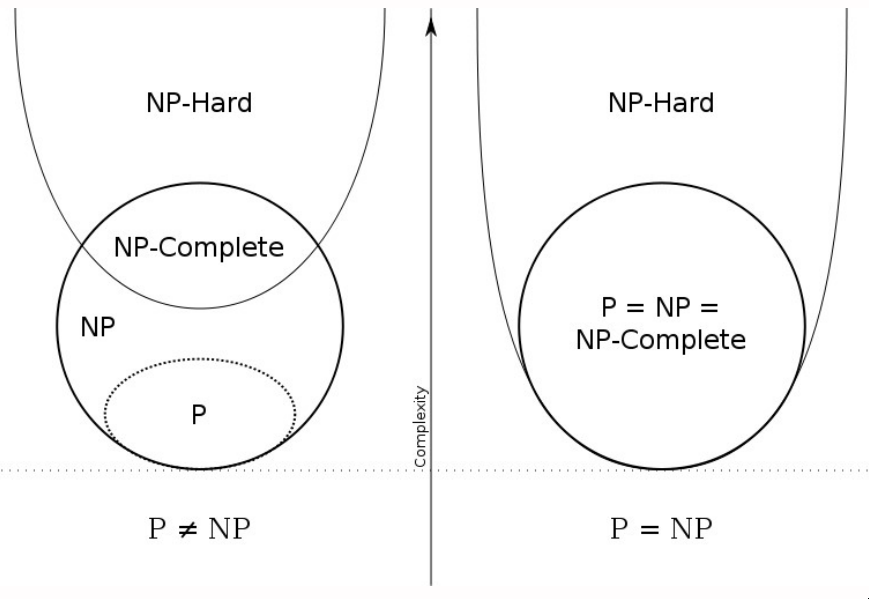
\includegraphics[width=0.6\textwidth]{pvsnp.png}
\end{center}

\begin{itemize}
    \item   \textbf{P} (Polynomial): Solvable in polynomial time. 
    \item   \textbf{NP} (Non-Deterministic Polynomial): Only \textit{verifiable} in polynomial time. 
\end{itemize}

\section{Searching \& Sorting}
\subsection{Keys \& Values}
Each object to be sorted can be considered to have a \textbf{key} \& a \textbf{value}, e.g. A Student has properties Name, ID, \& grade.

\subsection{Java Interface: Comparator} 
The \verb|Comparator| interface compares two objects to say which should come first. 
In Java, any class that implements \verb|java.util.Comparator| interface is only required to implement one method: 
\begin{lstlisting}[language=java] 
int compare(Object ob1, Object ob2); 
\end{lstlisting}

This returns a negative number if \verb|ob1| is less than \verb|ob2|, a positive number if \verb|ob1| is greater than \verb|ob2|, and \verb|0| if \verb|ob1| is equal to \verb|ob2|. 

\subsection{Java Interface: Comparable}
The \verb|Comparable| interface  compares a given object to another to see which object should come first. 
The two objects that are being compared must be of a class that implements \verb|java.lang.Comparable|, which has just one method to implement: 
\begin{lstlisting}[language=java] 
int compareTo(Object other); 
\end{lstlisting} 

Standard classes such as \verb|String| implement this.

\subsection{Insertion Sort} 
Consider sorting a bookshelf using \textbf{Insertion Sort}: 
\begin{enumerate} 
    \item   Remove the next unsorted book.
    \item   Slide the sorted books to the right one by one until you find the right sport for for the removed book. 
    \item   Insert the book into its new position once it is found.
\end{enumerate}

\begin{algorithm}
    \caption{Insertion Sort Pseudocode}
    \begin{algorithmic}
        \Require{$A[0 \dots N-1]$} \Comment{Unsorted Array}
        \Ensure{$A[0 \dots N-1]$} \Comment{Sorted Array}

        \Procedure{Insertion Sort}{$A[0 \dots N-1]$}
            \For{$ToSort \gets 1$ to $N-1$ Step 1}
                \State $Index = ToSort -1$ 
                \State $ToSortEl = A[ToSort]$ 
                \\
                \While{$Index \geq First$ AND $A[Index] > ToSortEl$} 
                    \State $A[Index+1] \gets A[Index]$ \Comment{Shuffle elements to the right}
                    \State $Index \gets Index - 1$
                \EndWhile
                \\ 
                \State $A[Index+1] = ToSortEl$ \Comment{Insert the element to sort in its appropriate place}
            \EndFor

            \State \textbf{return} $A[]$ \Comment{Return the sorted array}
        \EndProcedure
    \end{algorithmic}
\end{algorithm}

The worst case efficiency of Insertion Sort is $O(n^2)$. 
The best case efficiency of Insertion Sort is $O(n)$. 
If the array is closer to sorted order, the algorithm does less work, and the operation is more efficient.
This leads to a related algorithm: Shell Sort.

\newpage
\subsection{Shell Sort}
\textbf{Shell Sort} is more efficient than Selection Sort or Insertion Sort. 
It works by comparing distant items first, and works its way down to nearby items. 
The interval is called the \textbf{gap}. 
The gap begins at one half of the length of the list and is successively halved until each item has been compared with its neighbour.

Insertion Sort only tests elements in \textit{adjacent} locations - it might take several steps to get to the final location. 
Insertion Sort is more efficient if an array is partially sorted.
By making larger jumps, Shell Sort makes the array become ``more sorted'' more quickly.

\begin{algorithm}
    \caption{Shell Sort Pseudocode}
    \begin{algorithmic}
        \Require{$A[0 \dots N-1]$} \Comment{Unsorted Array}
        \Ensure{$A[0 \dots N-1]$} \Comment{Sorted Array}

        \Procedure{Shell Sort}{$A[0 \dots N-1]$}
            \State $Gap \gets floor(\frac{Gap}{2})$ \Comment{Round to the nearest odd number, as it's best with an odd-sized gap}
            \\
            \While{$Gap \geq 1$}
                \For{$ToSort \gets 1$ to $N-1$ Step 1}
                    \State $Index = ToSort -1$ 
                    \State $ToSortEl = A[ToSort]$ 
                    \\
                    \While{$Index \geq First$ AND $A[Index] > ToSortEl$} 
                        \State $A[Index+1] \gets A[Index]$ \Comment{Shuffle elements to the right}
                        \State $Index \gets Index - 1$
                    \EndWhile
                    \\ 
                    \State $A[Index+1] = ToSortEl$ \Comment{Insert the element to sort in its appropriate place}
                \EndFor
                \\ 
                \State $Gap \gets floor(\frac{Gap}{2})$
            \EndWhile
        \EndProcedure
    \end{algorithmic}
\end{algorithm}

The worst-case complexity of Shell Sort is $O(n^2)$.
However, this is because the gap is sometimes even which results in sub-arrays that include all the elements of an array that was already sorted.
To avoid this, we round the gap up to the nearest odd number which gives us a worst-case complexity of $O(n^{1.5})$.
Other gap sequences can improve performance a little more, but this is beyond the scope of this topic.

\subsection{Quick Sort}
\textbf{Quick Sort} is a divide-and-conquer algorithm. 
\begin{enumerate}
    \item   Firstly, it partitions the array into two sub-arrays that are \textbf{partially sorted}. 
    \item   Then, it picks a \textbf{pivot value}, and re-arranges the elements such that all elements less than or equal to the pivot value are on the left of the pivot, and all elements that are greater than 
            it are on the right.
    \item   The array is now divided into sub-arrays and a pivot value. 
    \item   This procedure is then repeated \textbf{recursively} for each sub-array, to further sort each of them.
    \item   When the algorithm has reached the level of a sub-array with just one element, that sub-array is sorted.
            All sub-arrays are sorted relative to each other, so the whole array is sorted when all the sub-arrays are.
\end{enumerate}

\section{Trees}
The data structures that we looked at previously placed data in linear order, but we sometimes need to organise data into groups \& sub-groups.
This is called \textbf{hierarchical classification}, where data items appear at various levels within the organisation.

In Computer Science, a tree is an abstract model of a hierarchical structure which consists of nodes with a parent-child relation. 
Trees have applications in organisation charts, file systems, programming environments, \& more.
A \textbf{tree} is a set of nodes, connected by edges. 
The edges indicate relationships between nodes.

Nodes are arranged in \textbf{levels}, which indicate the node's position in the hierarchy. 
Nodes with the same parent node are called \textbf{siblings}. 
The only node with no parent is the \textbf{root} node.  
All other nodes have one parent each.
A node with no child nodes is called a \textbf{leaf} node or an \textbf{external} node.
All other nodes are referred to as \textbf{internal} nodes.

A node is reached from the root by a \textbf{path}. 
The length of a path is the number of edges that compose it. 
This is also referred to as the depth of the node.
The \textbf{height} of a tree is the number of levels in the tree. 
The number of nodes along the longest path is equal to the maximum depth plus one.
Note that we talk about the depth of a node, but the height of a tree.

The ancestors of a node include its parent, grandparent, great-grandparent, etc.
The descendants of a node include its children, grandchildren, great-grandchildren, etc.
A \textbf{subtree} of a node is a tree that has that node as its root, including the node, all its descendants, and the arcs connecting them.

\subsection{Binary Trees}
A \textbf{binary tree} is one in which each internal node has at most two children (\& exactly two if it is a ``\textbf{proper}'' binary tree). 
The children of a node are an \textbf{ordered pair}.
We refer to the children of an internal node as the left child \& the right child.
Non-binary trees are termed general trees.

An alternative (recursive) definition for binary trees is a tree that is either just single node or a tree whose root has an ordered pair of children, each of which is a binary tree.

A \textbf{full binary tree} is one in which is a proper binary tree, and in which all the leaves are on the same level.
This is only achievable for certain numbers of nodes.
A \textbf{complete binary tree} is a binary tree which is full to the penultimate level and the leaves on the last level are filled frmo left to right.
This is achievable for any number of nodes.

The height of either a complete or full binary tree with $n$ nodes is log$_2(n+1)$. 

\begin{center}
    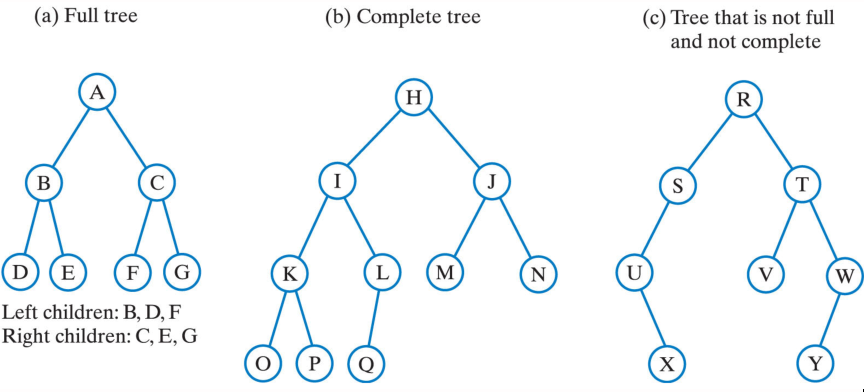
\includegraphics[width=0.7\textwidth]{binarytrees.png}
\end{center}

\subsection{Generics in Java} 
The \verb|< >| operators relate to the concept of \textbf{generics}. 
Generics are used to specify a specific type parameter for a generic collection class. 
This saves us from having to cast objects in methods such as \verb|add()|, \verb|set|, \& \verb|remove|.
This is a big advantage, as type checking is now done at compile time.
Without generics, compile-time type-checking is impossible, since we don't have a type specification for the list.
Other object-oriented programming languages have similar concepts, such as templates in C++.

\verb|ArrayList|s are part of the Java Collections framework, a standard library of pre-built data structures.
The underlying storage of an \verb|ArrayList| is an array. 
The \verb|ArrayList| class looks after resizing it as required.
\verb|ArrayLists| can be used with or without generics notation.

\begin{lstlisting}[language=Java]
// ArrayList code without generics: 
ArrayList words = new ArrayList();  // holds objects 
words.add("hello"); 
String a = (String) words.get(0);   // return type of get() is object, so must cast to String

// ArrayList parameterised to specifically hold Strings 
ArrayList<String> words = new ArrayList<String>(); 
words.add("hello"); 
String a = words.get(0);            // no cast needed
\end{lstlisting}

Creating a Generics collection: 
\begin{lstlisting}[language=Java]

public interface List<E> {
    void add(E x);
    Iterator<E> iterator();
}
public interface Iterator<E> {
    E next();
    boolean hasNext();
}
\end{lstlisting}

\section{Search Trees}
A \textbf{Search Tree} organises its data so that searching it is efficient.

\subsection{Binary Search Trees}
A \textbf{Binary Search Tree (BST)} is a binary tree with nodes that contain \verb|Comparable| objects. 
A node's data is greater than the data in the left subtree and less than the data in the right subtree. 
Usually, no duplicates are allowed. 

An \textbf{in-order} traversal of a BST will visit all nodes in ascending order.

BSTs are not uniquely structured - The structure of a BST depends on what node is chosen as the root of the tree and the order in which all the other nodes are added.

\bibliographystyle{unsrtnat}
\bibliography{references}
\end{document}
